\section{Development results}\label{sec:results}
\subsection{Historical benefit is family dependent}
Historical inverse affine correction reduces pooled RF MAE from 0.8993 to 0.7843 ppm and $P_1$ from 34.17\% to 28.86\%. Table~\ref{tab:historical} retains both family effects and their conditional resampling sensitivity. Figaro supplies 1,056 of 1,230 consensus exceedances (85.85\%) and 871 of 1,039 affine exceedances (83.83\%). Of the 191 net exceedances removed by historical affine correction, 185 are Figaro and six are FIS; the improvement is predominantly, not exclusively, Figaro.
\begin{table}[H]\centering\small
\caption{RF historical-only results. Family emphasis is a declared development extension; pooled results retain the original endpoint. MAE in ppm, $P_1$ in percent; brackets are conditional resampling intervals (length 10).}\label{tab:historical}
\setlength{\tabcolsep}{4pt}\begin{tabular}{lrrrrrr}
\toprule
Scope & Consensus & Affine & $H$ MAE & Conditional bounds & Raw $P_1$ & Affine $P_1$ \\ \midrule
Figaro & 1.5289 & 1.2742 & -0.2548 & [-0.3098, -0.1765] & 58.67 & 48.39 \\
FIS & 0.2697 & 0.2943 & 0.0246 & [0.0121, 0.0363] & 9.67 & 9.33 \\
ALL & 0.8993 & 0.7843 & -0.1151 & [-0.1424, -0.0770] & 34.17 & 28.86 \\
\bottomrule\end{tabular}\end{table}

\begin{figure}[H]\centering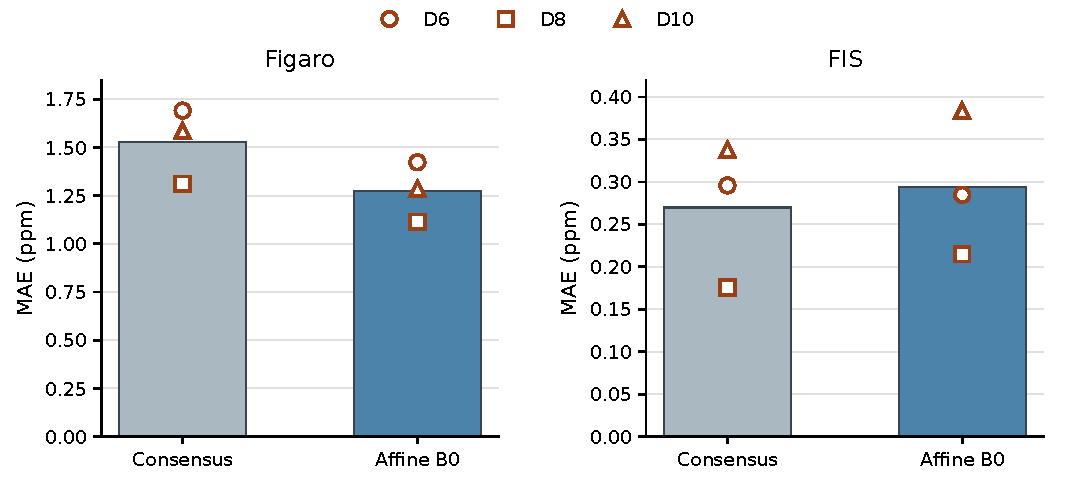
\includegraphics[width=.92\linewidth]{fig_1_historical_mae.pdf}
\caption{Development RF historical-only family MAE. Bars are equal-session means; outlined circles, squares and triangles show D6, D8 and D10, respectively. The Figaro and FIS panels use different vertical scales. Each family retains six correlated peer configurations on the same 100 exposures per session.}\label{fig:historical}\end{figure}
Table~\ref{tab:family} reports exact array-based family/session values. Figaro MAE improves on all three days. FIS MAE improves on D6 and worsens on D8/D10, although its strict exceedance count falls by two on each day. Endpoint directions therefore differ. The three affine lambdas have identical B0 predictions by construction and exact verification.
\begin{table}[H]\centering\small
\caption{Exact historical-only RF family/session values from prediction arrays; each cell has 100 exposures and 600 outputs. Counts are strict 1 ppm exceedances.}\label{tab:family}
\setlength{\tabcolsep}{4pt}\begin{tabular}{llrrrrr}
\toprule
Day & Family & Raw MAE & Affine MAE & $H$ MAE & Raw count & Affine count \\ \midrule
D6 & Figaro & 1.6909 & 1.4229 & -0.2680 & 366 & 298 \\
D6 & FIS & 0.2957 & 0.2847 & -0.0110 & 45 & 43 \\
D8 & Figaro & 1.3110 & 1.1139 & -0.1971 & 324 & 264 \\
D8 & FIS & 0.1757 & 0.2147 & 0.0390 & 39 & 37 \\
D10 & Figaro & 1.5850 & 1.2858 & -0.2992 & 366 & 309 \\
D10 & FIS & 0.3378 & 0.3836 & 0.0458 & 90 & 88 \\
\bottomrule\end{tabular}\end{table}

\FloatBarrier

\subsection{Additional references and forgetting}
Table~\ref{tab:incremental} compares B20 with each estimator's own B0, rather than attributing its historical advantage to new queries. All fifteen pooled RF B20 affine MAE changes are positive (adverse), although some lower-budget pooled point changes are favorable; the complete discrete-budget grid is retained. Under the envelope mask, changes are 0.0029, 0.0056 and 0.0115 ppm for $\lambda=1,.95,.90$. The native $.95$ comparator has MAE 0.7913 ppm and an incremental change 0.0070 ppm, with length-10 conditional bounds [0.0005, 0.0129] ppm. This tested coupled comparator does not improve pooled RF MAE. Exceedance directions, family effects and individual sessions differ; no universal statement about reference value follows.
\begin{table}[H]\centering\small
\caption{RF B20 changes from each affine estimator's common B0. Positive values worsen the endpoint. Conditional 95\% resampling bounds use block length 10. Last column counts sessions with a negative MAE change. All budgets, families and lengths are in the supplement.}\label{tab:incremental}
\setlength{\tabcolsep}{4pt}\begin{tabular}{llrrrrr}
\toprule
Estimator & Schedule & $I$ MAE & Conditional bounds & $I$ $P_1$ (pp) & Bounds (pp) & MAE $<0$ \\ \midrule
Affine $\lambda=1$ & Periodic & 0.0105 & [0.0072, 0.0142] & -0.11 & [-0.56, 0.28] & 0/3 \\
Affine $\lambda=1$ & Random & 0.0017 & [0.0006, 0.0030] & -0.09 & [-0.24, 0.06] & 0/3 \\
Affine $\lambda=1$ & Confidence & 0.0125 & [0.0081, 0.0178] & 0.03 & [-0.42, 0.42] & 0/3 \\
Affine $\lambda=1$ & Envelope & 0.0029 & [-0.0001, 0.0056] & 0.25 & [0.00, 0.53] & 0/3 \\
Affine $\lambda=1$ & Information & 0.0030 & [-0.0007, 0.0065] & 0.06 & [-0.19, 0.42] & 0/3 \\
Affine $\lambda=.95$ & Periodic & 0.0146 & [0.0102, 0.0191] & -0.19 & [-0.81, 0.33] & 0/3 \\
Affine $\lambda=.95$ & Random & 0.0024 & [0.0008, 0.0044] & -0.13 & [-0.33, 0.05] & 1/3 \\
Affine $\lambda=.95$ & Confidence & 0.0196 & [0.0123, 0.0283] & 0.25 & [-0.33, 0.83] & 0/3 \\
Affine $\lambda=.95$ & Envelope & 0.0056 & [-0.0001, 0.0109] & 0.19 & [-0.08, 0.56] & 0/3 \\
Affine $\lambda=.95$ & Information & 0.0070 & [0.0005, 0.0129] & 0.25 & [-0.19, 0.83] & 0/3 \\
Affine $\lambda=.90$ & Periodic & 0.0215 & [0.0146, 0.0278] & -0.14 & [-0.86, 0.50] & 0/3 \\
Affine $\lambda=.90$ & Random & 0.0042 & [0.0012, 0.0074] & -0.07 & [-0.38, 0.17] & 1/3 \\
Affine $\lambda=.90$ & Confidence & 0.0323 & [0.0193, 0.0473] & 0.28 & [-0.33, 0.89] & 0/3 \\
Affine $\lambda=.90$ & Envelope & 0.0115 & [0.0008, 0.0212] & 0.25 & [-0.39, 0.83] & 0/3 \\
Affine $\lambda=.90$ & Information & 0.0200 & [0.0056, 0.0337] & 0.78 & [-0.11, 1.81] & 0/3 \\
\bottomrule\end{tabular}\end{table}

\begin{figure}[H]\centering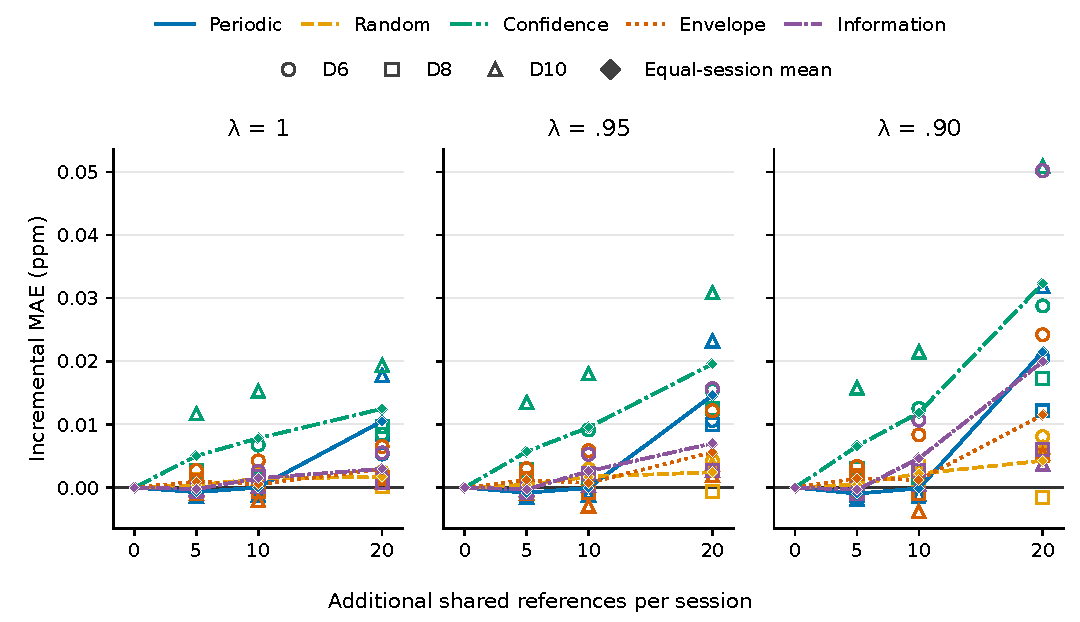
\includegraphics[width=\linewidth]{fig_2_affine_increment_mae.pdf}
\caption{Development RF pooled incremental MAE relative to each affine estimator's own B0, by update factor and schedule. Colors and line styles identify schedules; filled diamonds show equal-session means. Outlined circles, squares and triangles show D6, D8 and D10. All panels share one vertical scale; positive changes are adverse. Lines join evaluated discrete budgets only. Development-only conditional intervals and family values remain in the supplement.}\label{fig:incrementalmae}\end{figure}
\begin{figure}[H]\centering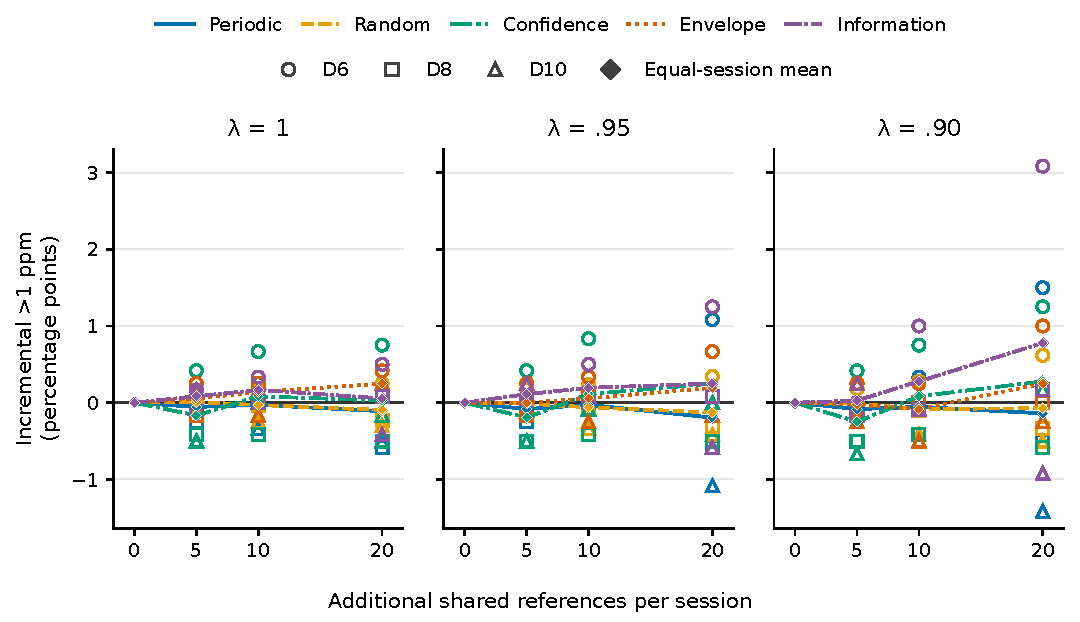
\includegraphics[width=\linewidth]{fig_3_affine_increment_exceedance.pdf}
\caption{Development incremental strict 1 ppm exceedance relative to own B0, in percentage points. Colors/line styles identify schedules, filled diamonds show equal-session means, and outlined circles/squares/triangles show D6/D8/D10. Panels share a vertical scale; positive changes are adverse. Lines join only evaluated budgets. MAE and exceedance can move in different directions.}\label{fig:incrementalp}\end{figure}
The cumulative envelope B20 estimate remains 0.7872 ppm and 29.11\% exceedance, compared with its own B0 at 0.7843 ppm and 28.86\%. Resampling intervals crossing zero are retained as conditional sensitivity bounds rather than interpreted as equivalence. Other schedules and block lengths, including unfavorable changes, remain visible.
\FloatBarrier

\subsection{Subset, support and upstream-model checks}
A concrete selection example is confidence B20 cumulative affine: unqueried MAE is 0.7403 ppm, but unchanged consensus on that same subset is 0.8580 ppm versus 0.8993 ppm on all exposures. The affine B0 MAE on those same unqueried exposures is 0.7243 ppm, so the positive-budget 0.7403 ppm is adverse against its own matched baseline. Selecting difficult exposures for purchase changes the unqueried population. Every subset now also has the estimator's own same-subset B0 and exact count, so subset selection and incremental prediction changes are distinguishable.

Concentration support and the 10\% relative tolerance are tabulated in Supplement S5 and the full numerical records. Both families have the same chamber-concentration support, while their errors differ. Reference-defined bands are evaluation diagnostics only.

A saved-input upstream-model sensitivity retains RF as primary. OLS historical affine MAE is 0.7678 ppm versus consensus 0.8652 ppm; ridge gives 0.9046 versus 1.0873 ppm. Under envelope B20, cumulative affine changes are $-0.0021$ and $-0.0025$ ppm for OLS and ridge. Native $.95$ changes are $-0.0037$ ppm for OLS and $+0.0039$ ppm for ridge. Thus the incremental pattern is model dependent. No model was refitted or promoted; OLS/ridge confidence uses peer MAD, unlike RF tree spread, and each model retains its own mask.

Paid queries in the last ten exposures and at exposure 100 are counted per run, then averaged over seeds and days (Supplement S6). Only exposure-100 purchases lack a subsequent scored prediction under reset; the other last-ten purchases can affect later outputs. All budgets remain charged.

\subsection{Containment is not assurance}\label{sec:boundresults}
Primary envelope-driven B20 midpoint width is 16.8528 ppm and containment 99.56\%, yet only 60 of 3,600 outputs (1.67\%) meet the conditional 1 ppm criterion. All 60 are unqueried: 60/2,880=2.08\%; queried outputs have none. No complete twelve-configuration unqueried exposure is assured under the original primary RF schedules. Sixteen primary B20 raw noncontainments occur without contradictions. Numerical consistency alone therefore does not establish containment.
\begin{table}[H]\centering\small
\caption{RF midpoint interval diagnostics on all exposures. Fractions average seeds within sessions and sessions equally; flags require a noncontradictory radius at most 1 ppm.}\label{tab:bounds}
\setlength{\tabcolsep}{4pt}\begin{tabular}{lrrrr}
\toprule
Schedule & $B$ & Width (ppm) & Contained (\%) & Flagged (\%) \\ \midrule
Historical only & 0 & 22.2412 & 99.78 & 0.61 \\
Periodic & 20 & 18.4844 & 99.50 & 1.28 \\
Random & 20 & 18.8071 & 99.50 & 1.19 \\
Confidence & 20 & 19.4958 & 99.28 & 0.78 \\
Envelope & 20 & 16.8528 & 99.56 & 1.67 \\
Information & 20 & 20.4082 & 99.72 & 1.28 \\
\bottomrule\end{tabular}\end{table}

The exact slope95/envelope B20 cross-tab reconciles 2,072 raw noncontainments: 749 contradictory outputs are contained by their descriptive hull, and 1,323 noncontradictory outputs remain outside their reported interval. This partition was checked by output identities. The complete 16-cell cross-tab, including zero cells and assurance, is in Supplement S7. Actual errors, rather than interval noncontainment alone, identify 503 false 1 ppm midpoint assurances among 2,287 assured outputs (21.99\%), and 503 among all 3,600 outputs (13.97\%). The 1,188 outside-and-assured entries are not themselves a false-assurance count. Primary midpoint bounds have 0/60 false assurances (0\%) and 0/3,600 overall, separately from their 16 noncontainments. The sensitivity remains a negative result. Broad primary bounds and failed narrower bounds are both retained.

The archived schedule grid contains repeated zero-budget runs that are numerically identical. After exact equality checks, the original grid reduces to one zero-budget run and 39 positive-budget masks per model/day/bound setting; the native schedules add 15 distinct runs across the evaluated models and days. These are computational identities on the same 300 physical development exposures, not additional experimental replication.
